\chapter{\ifproject%
\ifenglish Project Structure and Methodology\else โครงสร้างและขั้นตอนการทำงาน\fi
\else%
\ifenglish Project Structure\else โครงสร้างของโครงงาน\fi
\fi
}

ในบทนี้จะกล่าวถึงหลักการ, การนำทฤษฎีที่เกี่ยวข้องมาประยุกต์ใช้ และการออกแบบของระบบ

\makeatletter

% \renewcommand\section{\@startsection {section}{1}{\z@}%
%                                    {13.5ex \@plus -1ex \@minus -.2ex}%
%                                    {2.3ex \@plus.2ex}%
%                                    {\normalfont\large\bfseries}}

\makeatother
%\vspace{2ex}
% \titleformat{\section}{\normalfont\bfseries}{\thesection}{1em}{}
% \titlespacing*{\section}{0pt}{10ex}{0pt}

\section{การจัดเก็บข้อมูล}
โดยข้อมูลราคาหุ้นทุกตัวจะมีแหล่งที่มาจาก 2 ที่ก็คือ AlphaVantage และ Finnhub โดย AlphaVantage จะให้ข้อมูลย้อนหลังไป 2 ปี ส่วน Finnhub จะเอาไว้ใช้อัพเดท
ข้อมูลแบบ real-time ทุกๆ 1 ชม. เราใช้ MongoDB เป็น Database สำหรับจัดเก็บข้อมูลตลาดหุ้น และตัวชี้วัดทางเทคนิคที่เราต้องการใช้ เช่น RSI, MA เป็นต้น

ในตอนเริ่มตันนั้นเราดึงข้อมูลที่ต้องการมาจาก AlphaVantage ซึ่งก็คือข้อมูลตลาดหุ้นย้อนหลัง 2 ปีโดยใช้ API ของ AlphaVantage 
และเก็บข้อมูลลง MongoDB ด้วย Rust โดยมีการแปลงข้อมูลให้เป็นในรูปแบบข้อมูลตลาดของเราซึ่งก็จะประกอบด้วย
\begin{enumerate}
    \item ticker: ชื่อของหุ้นที่ทำการซื้อขาย เช่น AAPL/USD, IBM/USD
    \item open: เป็นราคาซื้อขายแรกที่เกิดขึ้นใน ช่วงเวลานั้นๆ
    \item close: เป็นราคาสุดท้ายที่เกิดขึ้นจากการซื้อขายสิ้นสุด ของช่วงเวลานั้นๆ
    \item high: การเคลื่อนไหวของราคาหุ้น ณ ระดับราคาสูงสุดในช่วงเวลานั้นๆ
    \item low: การเคลื่อนไหวของราคาหุ้น ณ ระดับราคาต่ำสุดในช่วงเวลานั้นๆ
    \item volume: ปริมาณการซื้อขายในช่วงเวลานั้นๆ
\end{enumerate}
จากนั้นในการ update ข้อมูลแบบ real-time เราจะใช้ MongoDB Scheduled Triggers ที่จะไปเรียกใช้ AWS Lambda ที่เราสร้างขึ้นมา โดยใน Lambda จะดึงข้อมูลจาก 
Finnhub มา update ซึ่งในการ update นี้ก็จะมีการ update ข้อมูลของตัวชี้วัดทางเทคนิคที่เราต้องการใช้ และ update ตัวชี้วัดทางเทคนิคของเราเองด้วย

\begin{figure}[ht]
    \centering
    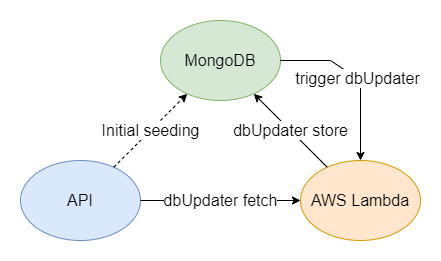
\includegraphics[scale=0.6]{images/db.png}
    \caption{โครงสร้างของการจัดเก็บข้อมูล โดนเส้นประคือทำครั้งเดียวในตอนแรกเริ่ม และเส้นทึบจะทำในทุกๆ ชม. โดยเป็นการเรียกใช้โปรแกรม dBUpdater ใน AWS Lambda}
    \label{fig:1}
\end{figure}

\section{เว็บเซิร์ฟเวอร์}


\section{การปรับแต่ง Fuzzy Logic ด้วย PSO}
เป้าหมายของเราในการปรับแต่ง Fuzzy Logic ที่ใช้สำหรับการสร้างตัวชี้วัดทางเทคนิคใหม่ของเรานั้น ก็คือการปรับแต่ง linguistic variables ต่างๆ ที่มีอยู่ fuzzy rules เพื่อให้
ตัวชี้วัดทางเทคนิคของเรานั้นสามารถสร้างกำไรได้มากที่สุดใน\emph{วิธีการเทรดที่เราใช้ปรับแต่ง} โดยเราจะใช้ PSO (Particle Swarm Optimization) ในการปรับพารามิเตอร์ที่ใช้
สร้าง linguistic variable แต่ละอัน โดยพารามิเตอร์ในการสร้าง fuzzy set นั้นจะแตกต่างกันไปตามรูปแบบของ fuzzy set 
ถ้าเป็นแบบสามเหลี่ยมก็จะมีพารามิเตอร์ดังที่เห็นในรูปที่ \ref{fig:2}

\begin{figure}[ht]
    \centering
    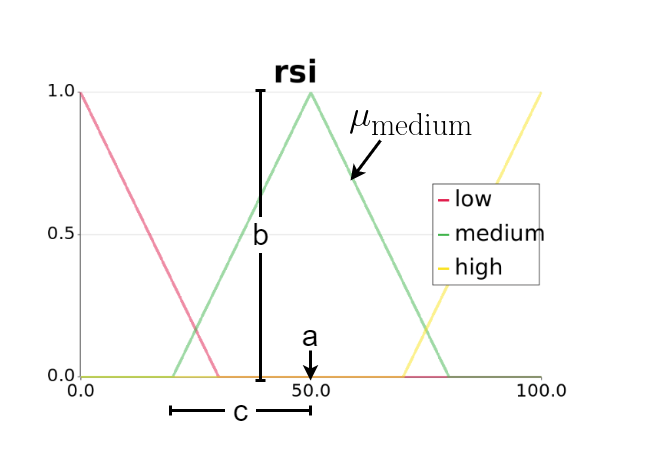
\includegraphics[width=0.8\textwidth]{images/linguisticv.png}
    \caption{linguistic variable และตัวแปรที่เราต้องการจะปรับแต่ง (ในรูปคือ $a, b, s$)}
    \label{fig:2}
\end{figure}

\subsection{กลยุทธ์ที่เราใช้ปรับแต่ง}
โดยในการปรับแต่ง Fuzzy Logic ของเรานั้นอันดับแรกเลยเราต้องเลือกกลยุทธ์การเทรดที่เราต้องการปรับแต่ง ให้มีผลต่อตัวชี้วัดทางเทคนิค ยกตัวอย่างกลยุทธ์การเทรด
เช่น มีเงินต้น 2000 บาท ถ้า buySignal มากกว่า 50 ให้เข้าซื้อด้วย 100 บาท ด้วย stop-loss ที่ 10\% และ take profit ที่ 20\% 
\subsection{Backtesting}
Backtesting คือการนำกลยุทธ์การเทรดที่เราเลือก ไปใช้กับข้อมูลในอดีตในกรอบเวลาที่ผ่านๆ มาเพื่อทดสอบว่ากลยุทธ์นั้นไปใช้ในตลาดจริงๆ ในอดีตแล้วได้ผลดีแค่ไหน
โดยเราสามารถเลือกกรอบเวลาที่ตลาดมีลักษณะคล้ายๆ กับในปัจจุบัน แล้วลองปรับเปลี่ยนและทดสอบกลยุธ์การเทรดนั้นๆ ได้เพื่อให้ได้ผลลัพธ์ที่เราต้องการ

โดยเราจะทำการ backtest ด้วยกลยุทธ์การเทรดที่เราเลือกมา แล้วเก็บข้อมูลการเทรดที่เกิดขึ้นทั้งหมดโดยแต่ละการเทรดจะมีข้อมูลดังนี้ 
\begin{itemize}
    \item เวลาที่เข้า position
    \item เวลาที่ออก position
    \item ราคาที่เข้าซื้อ
    \item ราคาที่ขาย
    \item จำนวนเงินที่จ่ายไป
    \item กำไรขาดทุนที่ได้ ($realizedPnl$)
\end{itemize}

\subsection{Objective Function}
เราจะใช้ Objective Function ที่คำนวณมาดังนี้ $f = \text{NP} + \text{MDD}$ โดย
\begin{itemize}
    \item {$\text{NP} = \frac{\sum_{i=0}^{n} p_i(\text{realizedPnl})}{\text{startMoney}}$ 
        คือ Net Profit ที่ได้จากการเทรดทั้งหมดโดยคำนวนจากข้อมูลการเทรดที่เราได้จากการทำ backtest โดย $n$ คือจำนวนข้อมูลทั้งหมด
        และ $p_i(\text{realizedPnl})$ คือข้อมูลตัวที่ $i$ โดยเอาค่า $\text{realizedPnl}$ มา 
    }
    \item {$\text{MDD}$ (Maximum Drawdown) โดยเราสามารถคิดค่านี้ได้โดยให้ $g(x) = \sum_{i = 0}^{x}p_i(\text{realizedPnl})$ 
    แล้ว $\text{MDD}' = \max_{r \in (0, n)} \left[ \max_{t \in (0, r)} g(t) - g(r) \right]$ และให้เราจำค่า $y = g(t)$ ที่ทำให้ได้ 
    $\text{MDD}'$ เยอะที่สุดไว้ แล้วจะได้ว่า $\text{MDD} = \frac{\text{MDD}'}{y}$
    }
\end{itemize}
